\documentclass{article}

\usepackage{graphicx}
\usepackage{tikz}
\usepackage{tikzsymbols}
\usetikzlibrary{calc,patterns,shapes.geometric}
\pagestyle{empty}
\usepackage[margin=0pt]{geometry}
\geometry{papersize={14in,12in}}

\def\centerarc[#1](#2)(#3:#4:#5){\draw[#1] ($(#2)+({#5*cos(#3)},{#5*sin(#3)})$) arc (#3:#4:#5);}

\begin{document}
	\begin{figure}
		\centering
		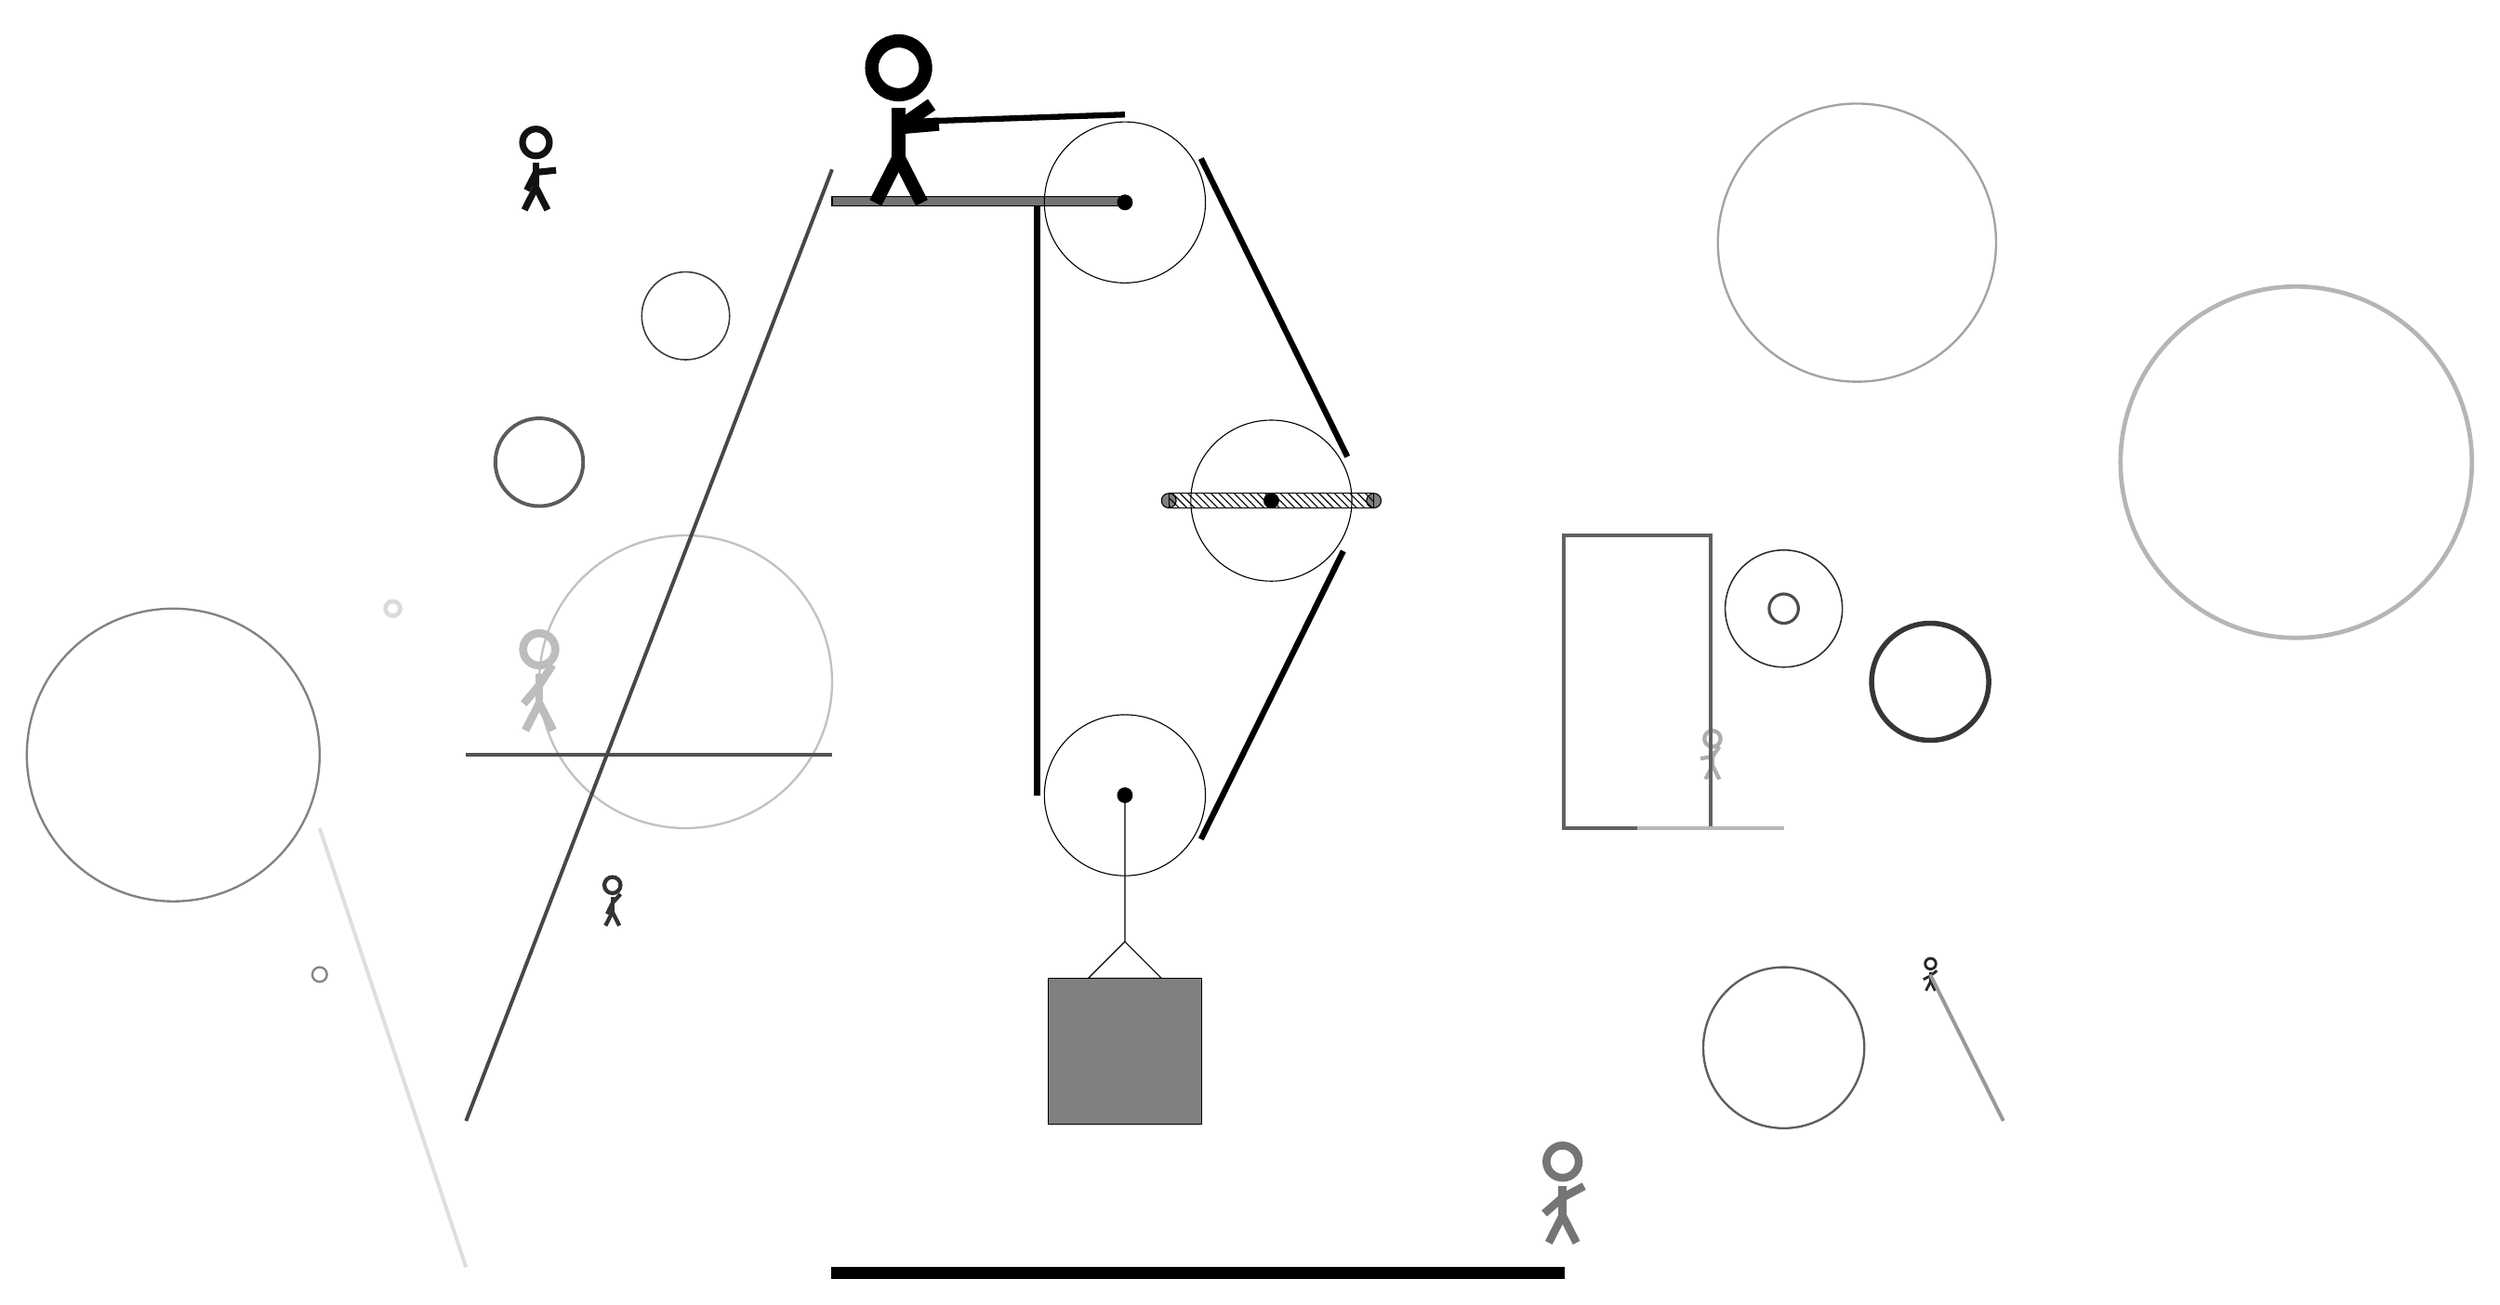
\begin{tikzpicture}
			%%%%% START %%%%%
			
			\draw[fill=black!55] (-2, 11.5) rectangle (2, 11.625);
			
			\draw (2, 3.45) circle (1.1);
			\draw[fill=black] (2, 3.45) circle (0.1);
			
			\draw [line width=0.4mm, color=black!70](11, 6) circle (0.2);
			
			\draw[line width=0.5mm, color=black!13](-7, -3) -- (-9, 3);
			\node[line width=0.7mm, color=black!80] at (-5, 2) {\Strichmaxerl[3][64][48]};
			\draw [line width=0.7mm, color=black!79](13, 5) circle (0.8);
			
			\draw [line width=0.3mm, color=black!63](11, 0) circle (1.1);
			\node[line width=0.5mm, color=black!32] at (10, 4) {\Strichmaxerl[3][9][56]};
			
			\draw [line width=0.5mm, color=black!64](-6, 8) circle (0.6);
			\draw [line width=0.3mm, color=black!24](-4, 5) circle (2.0);
			\draw [line width=0.6mm, color=black!14](-8, 6) circle (0.1);
			\draw[line width=0.5mm, color=black!68](-2, 4) -- (-7, 4);
			\draw [line width=0.2mm, color=black!77](-4, 10) circle (0.6);
			
			\node[line width=0.3mm, color=black!85] at (13, 1) {\Strichmaxerl[2][28][38]};
			\draw [line width=0.3mm, color=black!48](-9, 1) circle (0.1);
			\draw[line width=0.5mm, color=black!40](13, 1) -- (14, -1);
			\node[line width=0.4mm, color=black!93] at (-6, 12) {\Strichmaxerl[5][63][6]};
			\node[line width=0.2mm, color=black!54] at (8, -2) {\Strichmaxerl[6][41][28]};
			\draw [line width=0.3mm, color=black!36](12, 11) circle (1.9);
			\node[line width=0.4mm, color=black!26] at (-6, 5) {\Strichmaxerl[6][50][57]};
			\draw [line width=0.3mm, color=black!49](-11, 4) circle (2.0);
			
			\draw [line width=0.2mm, color=black!82](11, 6) circle (0.8);
			\draw[line width=0.5mm, color=black!62] (10, 7) rectangle (8, 3);
			
			\draw [line width=0.6mm, color=black!29](18, 8) circle (2.4);
			\draw[line width=0.5mm, color=black!28](11, 3) -- (9, 3);
			\draw[line width=0.5mm, color=black!72](-2, 12) -- (-7, -1);
			
			\draw (2, 11.55) circle (1.1);
			\draw[fill=black] (2, 11.55) circle (0.1);
			
			\draw[fill=white](4, 7.475) circle (1.1);
			\draw[fill=black] (4, 7.475) circle (0.1);
			\draw[fill=black!50] (2.6, 7.475) circle (0.1);
			\draw[fill=black!50] (5.4, 7.475) circle (0.1);
			\draw[pattern=north west lines, pattern color=black] (2.6, 7.575) rectangle (5.4, 7.375);
			
			\draw (2, 3.45) -- (2, 1.45) -- (1.5, 0.95) -- (2.5, 0.95) -- (2, 1.45);
			\draw[fill=black!50] (0.95, 0.95) rectangle (3.05, -1.05);
			
			\draw[line width=0.8mm] (0.8, 11.5) -- (0.8, 3.45);
			\centerarc[line width=0.8mm](2, 3.45)(180:330:1.2000000000000002);
			\draw[line width=0.8mm](3.0392, 2.85) -- (4.983, 6.7867);
			\centerarc[line width=0.8mm](4, 7.475)(390:325:1.2000000000000002);
			\draw[line width=0.8mm](5.0392, 8.075) -- (3.0392, 12.15);
			\centerarc[line width=0.8mm](2, 11.55)(30:90:1.2000000000000002);
			\draw[line width=0.8mm](2, 12.75) -- (-1, 12.65);
			
			\node at (-1, 12.65) {\Strichmaxerl[10][-175][35]};
			
			\draw[fill=black] (-2, -3) rectangle (8, -3.15);
			
			%%%%% END %%%%%
		\end{tikzpicture}
	\end{figure}	
\end{document}